\chapitre{Robespierre prend les commandes, le jeudi 28 juillet 2033 }{Vouloir atteindre le rêve d’une vie}{ ouvre parfois la porte à des raccourcis moraux pas toujours présentables dans les salons bienséants. Avec l’âge qui devient certain, il arrivera qu’on n’y regarde pas à deux fois avant d’avaliser une petite clause un peu particulière qui permettra néanmoins de se plonger dans son idéal avant qu’il ne soit trop tard. Pour le docteur Christian Bellavance, endocrinologue méconnu, chercheur n’ayant jamais eu l’occasion de faire partie d’une équipe sérieusement dirigée, homme de science n’ayant jamais pu voir son nom dans une publication crédible, l’atteinte de la cinquantaine avait été reçue comme l’annonce d’un cancer incurable avec amputations assorties sur une base hebdomadaire. Non pas qu’il aurait «voulu être un artiste, pour avoir le monde à refaire ».  }

Il n’était pas vraiment porté sur le sociopolitique et la misère humaine l’ennuyait. À 25 ans, il était prêt à tout. Sur le quai intermodal de la vie, il attendait qu’arrive le car de l’extraordinaire. Chaque matin, ses espoirs se ravivaient. Pourtant, à 30 ans, il avait commencé à agiter les bras, à envoyer des courriels de protestations aux autorités du transport existentiel. En vain. À 35, il avait finalement réalisé qu’aucun véhicule ne se présentait jamais, comme si les chauffeurs s’étaient mis, un jour, en grève permanente.

\begin{floatingfigure}[l]{35mm}
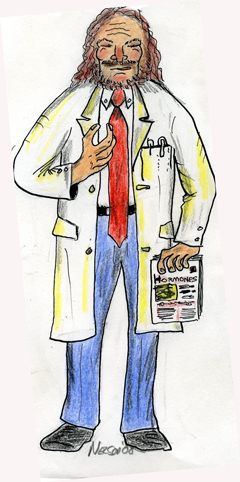
\includegraphics[height=60mm]{corps/chapitre17/img/personnage-bellavance.jpg}
\end{floatingfigure}

Alors lui, ce dépositaire d’une vie unique, potentiellement riche, ouverte à tout, une vie non renouvelable, non rebobinable, une vie de plus en plus monotone de médecin désabusé qu’il était en train de gaspiller au jour le jour dans une petite ville terne à côté d’une femme qui ne se promènerait jamais en string sur une plage brésilienne, lui qui n’avait jamais vu New York, Rio et Bangkok glissa tout doucement dans l’onirisme; il se mit à rêver de Delhi, Bali et Djara, à vouloir sentir, lui aussi, «les parfums de Chine» et le Sahara dans le souffle d’une belle. Il abandonna son quai et entra s’asseoir dans la taverne de l’imaginaire et de la fiction. Par personnages interposés, ceux de Jean-Marie Le Clézio, de Paul Auster, de Gabriel Garcia Marquez et de tant d’autres, il se créa des Saskatchewan qu’il quittait en train pour venir découvrir Montréal, des expéditions militaires en Égypte où il attrapait la vérole, une famille très étrange de Belleville dont il était l’aîné, une colonie de rats qu’il utilisait pour s’évader de la Bastille.

Mais il paraît que ceux qui aiment rêver passent leur vie à dormir. Voilà pourquoi, à 40 ans, il était devenu d’un ennui mortifère pour son entourage et qu’à 45, il s’était réfugié dans l’univers holographique quantique se modélisant des avatars en fonction des idéaux qu’il aurait tant souhaité vivre. Pourtant, le matin, quand il se regardait dans le miroir, il éprouvait la certitude, le temps d’une nanoseconde, «Time’s a loaded gun», qu’un jour, quelque chose se produirait, que sa vie si assommante, si mortelle, changerait. Qu’il vivrait vraiment. Envers et contre tous, il y croyait. Sinon, il se serait sûrement suicidé. Dieu sait qu’il en avait les moyens. N’était-il pas brillant et plein de ressources ?

Dans sa tête, il y avait constamment cette chanson essentielle de Brel qui trottait :

    Rêver un impossible rêve
    Porter le chagrin des départs
    Brûler d’une possible fièvre
    Partir où personne ne part

    Aimer jusqu’à la déchirure
    Aimer, même trop, même mal,
    Tenter, sans force et sans armure,
    D’atteindre l’inaccessible étoile

Alors quand à 51 ans, on lui avait parlé de ce projet de culture hormonale sur des corps cliniquement morts, il avait très rapidement fait taire sa conscience. Ces gens du ministère des Affaires gérontologiques avaient beau lui sembler de bien vils personnages, ils étaient LE pouvoir, ils avaient LES crédits et ils représentaient LA fin de sa triste vie inutile dans une petite ville ennuyeuse. En signant sur les pointillés, il faisait en sorte que désormais, il se passerait quelque chose, qu’il ferait les annales, que son nom serait associé, pour toujours, à un mini bond scientifique. Bref, Christian Bellavance s’était levé et avait quitté sa taverne.

Quant à sa «petite clause un peu particulière», il s’agissait simplement d’accepter de ne pas intervenir dans la mise en marché, la vente et la gestion financière du projet. Lui, il produirait les hormones, il trouverait des façons inédites pour en optimiser la fabrication et il gérerait l’aspect médical de l’aventure. On lui garantissait que tout excédent des revenus sur les dépenses serait versé au Centre afin d’améliorer le quotidien des bénéficiaires. À son âge et connaissant les humains, il n’y avait pas cru un instant. Mais, il avait enrobé ce doute certain de sept épaisseurs d’hypocrisie professionnelle, la spéciale résistante, celle qui se vend en contenants de deux litres dans toutes les forêts de gratte-ciel de la planète, et il était déménagé à Rimouski, laissant à Trois-Rivières épouse, ado, patients et voisins.

Dans des locaux du sous-sol initialement prévus pour les pensionnaires voulant se divertir en s’adonnant aux joies de la menuiserie légère, de l’électronique inoffensive, du tissage de catalognes, de la confection de lampes en papier de riz et de tous ces autres gossages de statuettes, le chercheur sur le retour d’âge s’était aménagé un centre de prélèvement, ainsi qu’un laboratoire, et on lui avait fourni le personnel nécessaire. Au bout de deux ans d’efforts, il avait récolté des résultats pour le moins spectaculaires. Il arrivait non seulement à obtenir le double de rendement par «corps souche» comme il appelait les semi-cadavres qu’on lui amenait, mais il réussissait à les maintenir en vie - un bien grand mot - trois fois plus longtemps qu’au départ de ses expériences. Il avait même un corps de vieille qui en était à son quatorzième mois de production.

Ce qu’on lui demandait surtout tournait autour de l’hormone humaine de croissance, la fameuse GH produite par la glande antéhypophyse, dite glande pituitaire antérieure. Le docteur Bellavance savait qu’on avait besoin de GH dans certains projets occultes de régénération ectopique d’organes vitaux, des projets dont dépendait le sort de certains patients très riches. Mais il savait surtout que certains laboratoires illégaux en achetaient de très grandes quantités pour en tirer des capsules de jouvence, des jujubes au goût de miel sensément capables d’agir comme agent anti-âge et antigras au risque des pires effets secondaires. Bien sûr, il y avait les hormones de synthèse, comme ces somatotrophines, lucratif fleuron du génie génétique de Monsanto. Mais on était loin de la qualité des vrais GH, même celles prélevées sur ces morts-vivants que le Centre lui livrait sur une base régulière.

Comme il n’était pas bête, il voyait bien l’écart entre les objectifs de production qu’il dépassait, mois après mois, et les résultats que Carl Michaud lui faisait remettre par Philippe Dauphin, sans jamais prendre le temps de lui expliquer quoi que ce soit. Il voyait bien qu’on l’assimilait à un exécutant sans grade et que les dividendes que son projet générait vraiment, on les lui cachait à coup sûr. En même temps, il constatait que l’ordinaire du CRG-BSL se détériorait sans cesse, ce qui signifiait, possiblement, que l’argent allait ailleurs.

Lorsque le sentiment d’être un rouage imbécile dans une magouille qu’il ne comprenait pas occupait toute sa tête, il se changeait les idées, cette fois non pas en se retirant dans son univers de fiction, mais en documentant, de façon maniaque, le déroulement de son entreprise. Ainsi, quand on lui donnerait le feu vert pour publier les résultats de sa recherche, il aurait tout en main. Il voyait déjà le titre : «Factor B : An Affordable Method to Optimize the Production of Human Hormones under Constant Clinical Supervision, by Professor Christian Bellavance, MD, FRCPC, FACP, Head of Research, CRG-BSL, Rimouski, Québec, Canada». Quel libellé ! «Factor B» ? Ne fallait-il pas brandir un magnifique «buzzword» à l’américaine pour référer à sa méthode ? «Factor B» sonnait bien, faisait professionnel et reprenait le «B» de Bellavance. Quant à «Professor», le titre se justifiait par le fait que le porteur avait été chargé de cours en techniques infirmières au Cégep de Trois-Rivières, durant … un semestre.

Tout cela pour dire qu’il fut à demi surpris quand il observa, sur une période de quinze jours, un employé de la direction des communications, Claude Sey, s’approcher de lui à la manière d’un requin faisant des cercles subtils. Il se doutait bien du sujet sur lequel le jeune homme finirait par l’entretenir, même si le prétexte était la préparation d’un document multimédia destiné à vanter les mérites du centre hormonal. Chattemite, le docteur se laissa manœuvrer, juste pour voir !

«Enfin, nous y voilà !» fut sa réponse lorsque Sey toucha au but pour la première fois.

- Quel est votre intérêt dans cette affaire ? Vous pouvez parler sans crainte, ici il n’y a ni caméra, ni micro, ni cafard, rien. Ça a fait partie de mes conditions quand on a construit.

Claude Sey plongea sans ambages.

- Je viens mettre mon nez dans vos tiroirs, docteur, parce que je ne sais pas trop quoi faire avec certaines informations.

- Quelles informations ?

- Les employés qui ont un bureau proche de celui de Philippe Dauphin – le mien est attenant - entendent parfois des bribes de conversation qu’il a avec Carl Michaud. D’une fois à l’autre, on finit par comprendre que votre projet serait une «machine à fric», une «mine d’or», la «passe du siècle». Mais en même temps, je m’excuse de devoir vous le répéter, vous seriez un «chercheur décollé de la réalité», un «naïf», un «lunatique» qui n’aurait aucune idée de ce qui se passe à deux pouces de son nez». Ça, c’est quand ils sont polis.

Bellavance ne sursauta pas.

- Vous n’avez pas répondu à ma question : quel est votre intérêt ?

- Si je lis attentivement les rapports que Michaud dépose au CA relativement à votre bébé, je vois qu’on y parle de «légers profits» ou de «profits prometteurs ». Guère plus ! Les entrées de fonds que vous générez, docteur, seraient à peine suffisantes pour couvrir vos coûts et pour justifier la continuation du projet. On est loin de la «machine à fric», de la « mine d’or» ou de la «passe du siècle» dont ils discutent entre eux. J’ai un gros doute à leur sujet; ça me ronge. Mon intérêt dans cette histoire ? Simplement de comprendre dans quelle galère je me suis embarqué en venant travailler ici. J’ai choisi le milieu gérontologique pour pouvoir contribuer, à ma façon, à améliorer leur sort misérable, pas pour cautionner une gamique.

- Et vous pensez, mon jeune ami, que je vais vous aider à vous faire une idée ? À apaiser votre conscience ?

- En vous parlant, j’ai couru le risque que vous soyez honnête. J’ai imaginé que vous saviez ce qui peut arriver, légalement, à des cadres qui boulechitent leur conseil d’administration, qui lui produisent des documents mensongers et qui brassent des affaires personnelles avec l’argent des contribuables.

Le médecin hésita, le temps de se fignoler une réponse à son goût.

- Nous allons arrêter cette conversation surréaliste, ici maintenant, monsieur Sey. Je pense vraiment que vous êtes mal servi par une imagination divagante à conséquences pathologiques. Prenez des vacances. Ça presse ! Au revoir monsieur.

Mais deux heures plus tard, il l’appelait en exigeant le mode confidentiel et lui donnait rendez-vous chez lui, le soir même.

Ce fut le début de plusieurs rencontres pendant lesquelles il fut possible de recouper l’information et d’obtenir des certitudes. Si, au terme, il manquait le montant réel des sommes détournées, on savait sans l’ombre d’un doute qu’une fraude était en cours. On savait notamment que le tandem Michaud-Dauphin avait confié la distribution des hormones à un ex-employé de Pete Barrett, un certain Julien «Djou» Dassilva. De plus, en passant des heures sur son terminal, Claude Sey avait trouvé des chiffres éloquents sur le marché des hormones naturelles. On savait maintenant qui les produisait, comment elles étaient expédiées, à qui elles se vendaient, en quelle quantité, à quelle fréquence et à quel prix. Même en coupant par dix la valeur marchande officielle, les rapports au CA auraient dû faire état de revenus de loin plus importants, compte tenu des quantités produites au sous-sol du CRG-BSL.

Ne restait plus qu’à déterminer la marche à suivre. Dans un premier temps, on rejeta l’affrontement direct avec la direction générale. On craignait de devoir se battre contre une organisation dont les ramifications s’étendaient en dehors du Centre. Le seul nom de Barrett avait de quoi faire frémir les moins timorés. On rejeta également l’idée de recourir à un membre du CA, un administrateur que l’on documenterait pour qu’il puisse poser des questions embarrassantes. Le seul qui semblait parfois faire preuve de résistance face à Michaud était Jean-Michel Desrosiers, un comptable de Rimouski qui, par ailleurs, était trésorier de comté pour le Parti libéral du Québec dont le patron était l’affreux Barrett. La police ? C’était courir au suicide professionnel. Encore ici, le dossier se serait retrouvé à plus ou moins brève échéance sur le bureau de Barrett. On décida plutôt d’étendre la base, de se mettre en situation de ne pouvoir compter que sur deux têtes, de former un groupe d’employés honnêtes et capables de se tenir debout, une sorte de «Comité du salut public» dont les membres auraient dépassé leur seuil de tolérance quant aux exactions et autres magouilles qui sévissaient dans l’établissement. Peut-être que là, en élargissant les ressources, les jeux de contacts, les possibilités d’entraide, on arriverait à quelque chose. Encore fallait-il être extrêmement prudent.

Mais qui dans une boîte aussi corrompue que le CRG-BSL pourrait correspondre au profil recherché ? Qui sinon certains marginaux comme Sébastien Larose, le dernier syndiqué de la fonction publique du Québec, Jipé Gendron, alias Tit-mononk, un résident en 2P qui représentait les bénéficiaires au Comité de déontologie, Robespierre Alcide, un tabletté statutaire qui passait ses journées à s’occuper d’on ne sait trop quoi, Vlado Markovsky, le directeur de l’informatique qui semblait en avoir plus qu’assez de la situation cybernétique, Shimoune Saint-Pierre, un homosexuel qui prenait plaisir à enquiquiner les pires éléments du Centre, Ophélie Marcotte, la jeune collègue de Saint-Pierre ou encore, Timothée Tardif, un CS-1 plein de compassion pour ses pensionnaires, mais dont tout le monde se moquait ?

- La clé à tout ce beau monde pourrait être Tardif, fit Claude Sey qui, avec l’aval du docteur, s’engagea à amorcer une manœuvre d’amorce circulaire auprès de lui, comme il savait si bien le faire.

Ce qui avait été fait, la semaine dernière, au sortir de la réunion mensuelle du Comité de déontologie.

Mais aujourd’hui, Christian Bellavance rumine dans son bureau avec. Comme à son ordinaire, du Brel comme trame sonore.

    Les vieux ne meurent pas, ils s’endorment un jour et dorment trop longtemps
    Ils se tiennent par la main, ils ont peur de se perdre et se perdent pourtant
    Et l’autre reste là, le meilleur ou le pire, le doux ou le sévère
    Cela n’importe pas, celui des deux qui reste se retrouve en enfer
    Vous le verrez peut-être, vous la verrez parfois en pluie et en chagrin
    Traverser le présent en s’excusant déjà de n’être pas plus loin
    Et fuir devant vous une dernière fois la pendule d’argent
    Qui ronronne au salon, qui dit oui qui dit non, qui leur dit : je t’attends
    Qui ronronne au salon, qui dit oui qui dit non et puis qui nous attend.

- Quand même !

Il regarde son terminal.

- Arrêt ! Autre arrangement ! Jazz ! Oui !

Chick Corea vient instantanément prendre la relève de l’immortel Wallon.

Débarrassé de sa distraction, le docteur comprend que la conjoncture s’est un peu complexifiée. Sey a été congédié; il n’a plus accès au Centre. Quant à Tardif, il n’a voulu rien entendre la veille. Mais il y a ce grand noir, cet Alcide, et cette pédale, ce Saint-Pierre, qui, à en croire Sey, auraient la confiance du chef de section. Et il y a les flics dans la boîte depuis hier ! Il y aura sûrement enquête. Michaud et Dauphin doivent être sur les dents. Le moment d’agir, du moins d’élargir le cercle pourrait être bon.

Puisqu’il faut battre le fer quand il est chaud, le chercheur quitte l’air glauque de son antre et monte vers la cafétéria. L’heure du petit déjeuner est presque finie et Saint-Pierre ne semble plus servir sa saloperie de manger mou. Il est même en train de discuter le bout du gras avec Alcide. Dans le vaste réfectoire, quelques vieillards flânent, des bénévoles ramassent les traîneries, d’autres nettoient la fontaine, essuient les dessus de table et replacent les chaises. À cette heure, se dit Bellavance, le conciliabule devrait bientôt se terminer. Le mieux est d’attendre dans le couloir, mine de rien, espérant voir apparaître l’un ou l’autre, ou les deux.

Bingo ! Voilà le colosse à la profession inconnue qui se pointe.

- Monsieur Alcide, le hèle-t-il.

Robespierre se retourne.

- J’ai bien l’honneur de porter ce nom. Et vous, monsieur, vous êtes ce docteur Bellavance qui travaillez au sous-sol pas trop loin des Tontons Macoutes, ces gens inquiétants qu’on surnomme ici Papyblues, mais que moi j’appelle Tontons Michauds.

- Je vois que vous faites dans l’humour noir, monsieur Alcide …

- Ouh ! qu’elle est cherchée celle-là !

La partie ne sera pas facile, oh que non !

- Bon, trêve de mondanités, je n’irai pas par quatre chemins. Hier j’ai essayé de dire certaines choses importantes à votre ami, monsieur Tardif, mais il n’a pas voulu les entendre. C’est dommage !

- Par les temps qui courent, Timothée en a plein les bras, le pauvre. Il ne sait plus trop où donner de la tête.

- Remarquez, ces choses, je pourrais vous les révéler à vous, vous en feriez ce que bon vous semble. Et, croyez-moi, vous serez en mesure de convenir que je ne vous aurai pas fait perdre votre temps.

- Quelles choses ?

- Mon bureau est un des rares endroits de ce centre, monsieur Alcide, où on peut parler sans danger. Passez me voir quand vous le voudrez.

- J’ai des disponibilités, maintenant.

- Dans ce cas, si vous voulez me suivre.

Quand, une demi-heure plus tard, Robespierre remonte aux étages, il a un topo complet en tête, celui d’une machination bien installée à la direction générale, où le docteur Bellavance fait figure de dindon de la farce. Quelques mots lui viennent à l’esprit dont exaction, gamique, concussion, tripotage, combine et, son préféré, prévarication.

- Madame Bellow, vous semblez en grande forme ce matin, fait-il en direction de l’ex-bibliothécaire occupée à fournir en livres, une quinquagénaire d’assez fraîche date qui, juchée sur une chaise, emplit la tablette du haut.

Dès le lendemain de l’affectation de Bea Bellow chez l’administrativement inutile Robespierre Alcide, des étagères en métal bêtement entreposées au sous-sol lui avaient été livrées, une gracieuseté du tout aussi inutile Sébastien Larose qui était copain-copine avec la responsable du mobilier, l’immémoriale Louise Lavoie. Rien n’échappait au contrôle de cette ancienne noceuse recyclée, avec responsabilités gestionnaires, dans le bric-à-brac institutionnel; ni les chaises bancales, ni les bouts de planche non utilisés, ni les tables de travail désaffectées, rien ! Aucun cadre décoratif, restant de peinture, chariot et téléviseur, aucune patère, tablette, retaille de tapis, poignée, serrure électronique et autre crédence, ne lui étaient étrangers. Quand elle entrait dans une officine, l’occupant avait l’impression qu’elle en connaissait intimement chaque objet et qu’il pouvait s’en faire déposséder en un clin d’œil.

- Le vrai pouvoir, aimait-elle répéter, ce n’est pas d’occuper le bureau du directeur général, mais d’en contrôler le mobilier ! Car privés de chaise, les trous de culs deviennent vulnérables !

Les mains sur les hanches, le sportif poursuit ses politesses.

- Et vous, madame Lavoie, vous êtes venue aider madame Bellow ? Quelle gentillesse ! En plus, vous me semblez toute primesautière.

- Primesautière, de quossé ?

- Frétillante, pimpante, fringante ?

- Faut ben. Dites donc vous, vous en avez donc b’en des livres ? Les avez-vous tout’ lus ?

- Oui ! Mais là, maintenant, j’en cherche un d’Henri Amouroux.

Bea Bellow, cesse un instant son petit manège et tape des mains.

- Là-bas, deuxième tablette, vers la gauche, reliure jaune.

Robespierre a tôt fait de repérer le bouquin, de le feuilleter fébrilement, d’émettre un grand ahhh! et de scribouiller sur une feuille qu’il se dépêche d’aller coller à sa porte. On peut y lire :

    Le drame des dictatures, c’est qu’elles donnent toute licence aux malades mentaux, aux mégalomanes, aux méchants, aux malhonnêtes gens d’aller jusqu’au bout de leur folie, de leur mégalomanie, de leur méchanceté, de leur malhonnêteté.

- Aussi bien afficher ses couleurs ! sourit le gaillard en se tapotant la boucle d’oreille.

Sans délai, il entre en communication avec Marie-Odile Tremblay.

- Écoute, je me demandais, comme ça, si c’était possible de te parler sans gadget, ni cafard, ni témoin, genre maintenant, tout de suite ? J’ai un truc qui va sûrement t’intéresser.

- C’est possible, t’as juste à passer à mon bureau.

Le ton est maussade. Il tente d’égayer.

- J’ai suffisamment de gènes afro-américains dans le corps pour savoi’ que les pauv’es noi’s ont inté’êt à ne pas fwéquenter les commissa’iats de flics !

- C’est ça, fais le cave !

Pas en forme, la matrone !

- J’ne rigole pas. Dis, pourquoi on n’irait pas prendre l’air, en haut, sur le toit ? C’est agréable, il fait beau, y a des chaises, des balançoires, de belles fleurs, le décor parfait pour jaser de mes affaires ?

- Coudon, t’es-tu parano, toi ?

- Je te prends peut-être dans un mauvais moment ? Je peux te rappeler plus tard ?

Marie-Odile se revoit, hier soir, retourner chez elle, seule, défaite, frustrée, en colère, jalouse à en avoir mal au ventre, une douleur moins supportable encore que celle de ses menstruations difficiles. Elle se revoit vouloir ouvrir sa porte d’appartement à grands coups de pieds et se retenir in extremis. Elle se revoit en train de maudire ce Timothée, l’idiot du village sur qui elle est tombée, et qui, malgré sa dégaine, la rend déjà malheureuse. Évidemment, si elle était moins possessive, défaut épouvantable, elle le sait, qui, à ce jour, a ruiné le peu de relations amoureuses qu’elle a connues, elle n’en aurait possiblement rien à glander. Effectivement, pourquoi cet homme ? Il y en a pourtant bien d’autres. Parce qu’il est un homme avec tout l’attirail nécessaire ou parce qu’il est Timothée, avec toute sa gentillesse de perdant ?

- Bof !

- Tu ne perdras pas ton temps.

Pourquoi pas !

- Bon ! C’est comme tu veux. Je monte.

- Pas de gadgets électrochoses ?

- Pas de gadgets.

- Promis ?

- Promis, bougonne celle que les employés surnomment la Bitch.

Il faut à Robespierre, écrasé dans une chaise de parterre, ses longues jambes sur une autre, un bon cinq minutes pour bien raconter la fraude dont se dit exécutant involontaire le docteur Bellavance. Marie-Odile, assise les fesses serrées sur le rebord d’une table, semble réfléchir.

- Il t’a fourni des preuves ?

- Des rapports au CA qui n’ont rien à voir avec sa vraie production. Des déductions. De quoi intéresser les enquêteurs. Ça sent la chiotte en train d’se boucher.

- Pourquoi tu me contes ça ?

Si l’âme du sieur Alcide était aussi limpide que celle d’un nouveau-né, il répondrait «pour mieux de sauter, mon enfant !» Mais voilà, Robespierre est un adulte de 2033 qui accomplit son sacerdoce quotidien dans le remugle du CRG-BSL. Il parle donc d’une mainmise sur l’établissement par une clique de malfaiteurs, dont les éléments les plus visibles sont Carl Michaud et Philippe Dauphin. Ce sont des gens qui grattent partout pour économiser, ce qui leur permet de mieux empocher. Tout cela, bien entendu, se fait au détriment des bénéficiaires à qui on a presque tout coupé. Le gymnase a été trafiqué en salon des employés, le centre de bricolage en atelier pour le docteur Bellavance, la piscine condamnée, la très belle terrasse sur le toit, interdite, la climatisation réservée aux deux étages administratifs, le personnel de nuit charcuté à sa plus simple expression, les vieux logés en dortoirs 2P souvent obligés d’aller changer les couches dans les salles palliatives, sans parler de cette saloperie de Nutrisuz, le foutu manger mou que fait préparer l’ignoble Amédée Chicot, un autre parasite associé à la magouille. Or, avec le trafic présumé des hormones de culture, c’est à la veille de sauter; quelqu’un quelque part va finir par tout comprendre. Et le jour où cette révélation frappera, dans une semaine, dans un mois, dans un trimestre, beaucoup de hauts gradés auront à choisir leur camp et à montrer patte blanche.

Le problème est simple :

- Si on attend que ça pète, parce que ça va arriver, on ne pourra rien pour aider Timothée qui est aux prises avec une histoire kafkaïenne.

- Je te suis pas.

- Je dis que si on se met en mode proactif, qu’on fasse crever l’abcès, on n’sera pas trop loin des commandes quand viendra le temps de sauver Marie Rioux et Romain Tardif.

La fille Tremblay voit passer devant elle l’image de ses propres parents, celle de son père usé, mal en point, celle de sa mère, angoissée, craintive.

- Qu’est-ce que t’entends par «faire crever l’abcès» ?

\begin{floatingfigure}[l]{30mm}
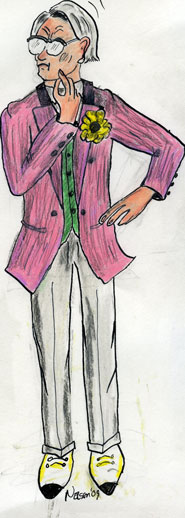
\includegraphics[height=60mm]{corps/chapitre17/img/personnage-carl.jpg}
\end{floatingfigure}

- B’en, on commence à avoir en main une couple de dossiers faciles à documenter et pouvant mener ces salauds au gibet. Il suffit de bien s’en servir ! J’imagine Carl Michaud, la corde au cou, avec son veston vieux rose, ses lunettes d’intello, sa ‘tite coupe de cheveux kioute et ses godasses de banquier 1900. Bordel !

Elle le regarde, les yeux plus plissés que la normale, ce qui est assez près de la grimace.

- Une «couple de dossiers» ?

Robespierre avait prévu le coup.

- OK, je vais t’asséner l’essentiel d’une deuxième histoire à relents de fosse septique.

Y prenant autant de plaisir que s’il avait été en train d’amuser des enfants à l’Heure du conte, l’arrière-petit-fils de l’inventeur du Petepano narre à l’Ilsa-de-Timothée l’invraisemblable découverte de Shimoune Saint-Pierre, ajoutant, hypocrite, force détails scabreux, incluant la dysfonction érectile de Pete Barrett.

- On a plein de clips qui nous présentent, bien en santé, les parents pourtant décédés du Gros Turcotte. On sait que ce pavillon est financé par l’État et qu’il abrite des illégaux intimement «plogués» sur cet immonde goret.

Robespierre s’est emporté et Marie-Odile est sidérée.

- Astie !

- Je t’le fais pas dire, ma belle !

Si l’expression «roucouler des yeux» était consacrée, quelqu’un en autorité l’aurait consignée dans un ouvrage officiel comme signifiant «Mouvement soutenu d’une paire de grands yeux noirs destinés à renforcer d’une façon frôlant l’indécence, le non-dit sexuel de propos relatifs à autre chose.» Bref, malgré l’orientation de la conversation à donner la chair de poule, Robespierre devise la bite sous le bras. On ne se refait pas.

Au même moment, Timothée est assis à l’arrière d’un taxi en train d’expliquer au chauffeur que pour la première fois de sa vie, il est en retard au boulot.

- Grosse soirée, mon jeune homme, ausculte Jawad Kebbaj.

- Je viens de me réveiller; j’ai même pas pris l’temps de manger.

Le bonhomme fouille dans un sac, sur le siège à sa droite, et en ressort une clémentine.

- Tiens, mange au moins ça.

- Euh, je sais pas si je dois …

- Écoute mon jeune homme, la clémentine est le cadeau du Maroc à l’humanité entière. Si tu veux insulter un Marocain, refuse la clémentine qu’il t’offre. P’is un Marocain insulté, c’est très très dangereux. Ouh la-la !

- En ce cas, je vais m’incliner. Merci monsieur Kebbaj.

L’agrume en main, Timothée entre au Centre et s’enligne vers les ascenseurs. Ce faisant, il croise le gros Lavoie, canaille sévissant comme préposée au 6e Nord. Le taupin le regarde, l’air narquois.

- Bonne nouvelle pour toi, le Motté, t’auras p’us à nous ramener la mére Morency.

Comme le CS-1 ne réagit pas, l’obèse enchaîne.

- On s’est écœuré et on l’a crissé en SP. A va décoller dans un sac zippé à la prochaine cérémonie. L’incinérateur, bye-bye ‘stie !

Instantanément, Timothée se rue sur Lavoie. Vociférant tel un schizophrène en crise, il le pousse sur le mur et le repousse à chaque fois que le misérable tente de rétablir sa dignité. De toute évidence, il a perdu le contrôle de ses émotions et, dans ses hurlements, on peut sentir l’expression de son impuissance face à une décision définitive prise un étage en haut du sien, une décision sur laquelle il n’a aucun droit de regard. C’est Shimoune Saint-Pierre qui, arrivé à la course, se saisit du forcené, un forcené dont la colère est telle qu’il doit fermement l’emprisonner par-derrière, dans ses bras puissants, et l’entraîner à grand fracas vers la cafétéria. Inutile de dire que dans le couloir, plus personne ne bouge ni ne parle et que tous vont se souvenir longtemps de cette violente éruption de rage sourde.

- Câlisse, Shimoune , ils vont tuer madame Morency, crie-t-il en déplaçant une table d’un coup de pied, ce qui, dans un vacarme amplifié par la vastitude du local, fait tomber deux chaises.

Quelques vieillards désœuvrés se dépêchent de filer.

Comme il se doit, la patience à toute épreuve de la «Grande folle du manger mou» arrive à calmer le malheureux chef de section, à le faire se ressaisir et, surtout, à le faire asseoir.

- Veux-tu une limonade ? Un thé ?

- Ça n’a plus de maudit bon sens, Shimoune, chigne son ami. Faut absolument faire quelque chose. Crois-moi, j’vas tout casser, j’vas tout arracher. C’est pas vrai que j’vas les laisser faire ça.

Le préposé au Nutrisuz tapote son dispositif personnel polyvalent.

- Allô dieu d’ébène ? As-tu une minute ? Oui ? Peux-tu descendre ici à la cafétéria ? Timothée a besoin d’aide; c’est sérieux. Il est arrivé un bordel. Oui mon chou, une bagarre. Ne-non ! Moi ? J’ai encore une demi-heure à tirer, y a du bon manger mou à servir, miam-miam ! Merci. Je t’attends, chou.

Sur le toit du Centre, Robespierre s’excuse auprès de Marie-Odile.

- Il est arrivé quelque chose à Timothée, faut que j’aille le chercher à la cafétéria.

- Quoi ?

- Une bagarre. Il est un peu, euh, désorganisé.

Si la femme flic est immédiatement allumée par le mot «bagarre», phénomène excessivement rare dans un établissement gériatrique, la femme tout court l’est encore plus par le fait qu’il s’agisse de Timothée, cet éternel perdant qui l’a fait rager hier soir.

- Je te suis.

Quand il les voit arriver, Timothée regarde Shimoune, secoue la tête et se lève. Il a compris. En silence, sans un regard pour Marie-Odile, épreuve qui lui semble infranchissable, il serre de près ses amis vers l’ascenseur. Au 5e, ils foncent tous trois vers le bureau de Robespierre, sans s’occuper de Ronnie Ross qui veut parler de l’Illuminé – «il a fait un ACV» - ni du vieux Jean Saint-Gelais qui, à l’instar de ceux qui savent des choses sans les dire, arbore un rictus entendu, même s’il n’a jamais vraiment su grand-chose.

D’un commun accord, Béa Bellow et Louise Lavoie laissent entrer les trois envahisseurs et se glissent silencieusement vers le couloir.

L’agente de sécurité fouille dans son bermuda et finit par retrouver son petit zinzin noir sur lequel, du pouce, elle exerce une pression.

- Tout est maintenant brouillé. À c’t heure, raconte ce qui s’est passé.

- J’ai pété ma coche, lui répond Timothée. Le gros Lavoie m’a annoncé avec le sourire, qu’ils avaient placé madame Morency en SP et qu’elle serait gazée et incinérée à la prochaine cérémonie de groupe. Ça se peut pas ! Faut que j’arrive à empêcher ça.

Robespierre s’écrase dans son fauteuil et, les yeux fixés au plafond, émet un puissant bâillement.

- OK, trop c’est trop ! On clenche !

Il baisse les yeux vers Marie-Odile.

- T’es avec nous ?

- C’est qui, ça nous ?

- Pour l’instant, Timothée, Shimoune, moi. Tantôt, on va rajouter le docteur Bellavance et Claude Sey.

- On clenche comment ?

- C’est à voir, faut en jaser. T’es une experte en sécurité, tu peux sûrement nous aider.

- Moi ?

- B’en oui !

L’air renfrogné que la femme flic arborait jusque-là semble s’estomper.

- Faut que je voie vraiment le dossier qu’a le docteur Bellavance. Si c’est ce que tu dis, s’il y a matière à porter des accusations au criminel, c’est certain que j’embarque.

Robespierre brandit ses deux pouces en avant de lui.

- Yes !

Tous trois conviennent alors de rencontrer le médecin, idéalement chez lui, question de se faire une idée finale et, de là, se définir une stratégie d’attaque. Les humains étant ainsi faits, les gestes décisifs sont toujours posés par une infime minorité, des gens qu’on appelle leader, fonceur, bélier, chef, boss, capo, édile, adjudant-chef, maître, producteur, propriétaire, tennô, padrino, président, pape, directeur, foreman, caudillo, ministre, prédicateur, meneur, auteur. Mais ici, ils ont pour nom Robespierre Alcide, monument de force et de sagesse sur qui deux paires d’yeux sont fixées. Ce que voyant, l’armoire à glace pitonne sa boucle d’oreille.

- Docteur Bellavance, ici Robespierre Alcide. Peut-on parler de façon confidentielle ? Merci. Dites, je suis avec des amis et nous souhaiterions nous entretenir avec vous. Auriez-vous du temps, ce soir ? Oui ? Parfait. D’accord. Ça marche, 19h30 chez vous. Oui. Nous serons quatre. Ah ! Timothée Tardif, Shimoune Saint-Pierre et Marie-Odile Tremblay. Oui, l’agente de sécurité. Non, pas de problème. Je vous le dis. Parfait. Au revoir, docteur.

Il se recule dans sa chaise et étire ses longs tentacules.

- C’est parti !

S’il le pouvait, il prendrait Timothée dans ses bras et lui jurerait que plus personne ne pourrait désormais faire brûler de petits vieux, les nourrir à la soupane chimique, les vêtir comme des cloches, les traiter comme des demeurés. Il lui promettrait que ses parents, Marie et Romain, seraient délivrés de leur sous-sol poussiéreux, qu’ils pourraient vivre au grand jour sans devoir aller se cacher avec les autres sur l’île d’Anticosti. Il l’assurerait que les méchants qui commandent l’établissement seraient traqués, arrêtés, condamnés et écroués dans la plus humide des geôles en compagnie des Papyblues et autres Tontons Michauds, que le gros Turcotte serait traîné sur le banc d’infamie, puis accroché par le cou aux fourches patibulaires avec les boyaux du fraîchement éviscéré Pete Barrett. Mais on est en public, un public aux yeux inquisiteurs, plissés et, quelque part, bleus, dont la porteuse en uniforme de la Sécu semble en réflexion carabinée.

- J’m’en vais me coucher à la maison, soupire Timothée. Y a rien à faire avec moi, aujourd’hui.

- C’est correct, mon ami, repose-toi bien. J’vais passer te prendre à 19 h.

Dans le couloir, Ronnie Ross finit par le rattraper.

- Motté ? Je fais quoi avec l’Illuminé ? J’l’envoie en SP ?

- Non câlisse ! On n’enverra plus jamais personne se faire incinérer ! Fie-toi sur moi, Ronnie !

Ce dernier réalise que son chef, parvenu aux ascenseurs, n’est plus ce bon vieux Motté auquel il a été habitué. Il lui crie :

- Oui, mais je fais quoi avec ?

- T’appelles les secours, tu le fais soigner, comme un être humain !

Le préposé n’en croit pas ses oreilles. Mais il est trop tard, Timothée est déjà disparu.

Quand Robespierre passe le prendre à 19 h, le fils Tardif a l’impression que cinquante millions de caisses de clémentines marocaines lui sont passées sur le corps, même s’il a dormi un bon cinq heures. Mais il est serein, presque heureux. C’est qu’en se réveillant, il s’était fait un café et était descendu juger de l’état des choses chez ses parents. Stupéfait de ne pas entendre Gazou gronder comme un enragé, il en avait vite compris la raison en apercevant Béatrice en train de parler avec sa mère. Depuis quand y était-elle ? Il n’avait pas osé s’informer, se contentant d’en éprouver un grand bonheur. Il avait salué, puis retourné son sourire à la belle infirmière et, affreusement gêné, était reparti chez lui.

En arrivant devant la résidence du médecin, ils remarquent Marie-Odile dans sa voiture électrique qui les attend, avec Shimoune appuyé nonchalamment, les coudes sur le toit.

- Dieu du ciel, madame, comme ce soleil de fin de journée convient à votre carnation et à la dorure de vos cheveux. Jusqu’à la fin de mes jours, je serai redevable à l’astre de vie d’un tel spectacle.

La femme flic sourit presque au géant.

C’est Claude Sey, jeune idéaliste fraîchement congédié, qui, en se servant du quanticordi de la maison, se fait un devoir de présenter à Marie-Odile l’accablant dossier qu’il a accumulé. Puis, d’un commun accord, Shimoune relate sa ballade bicoise menant à la découverte d’un refuge pour illégaux hautement subventionné. Il a des clips et des photos. Autrement dit, résume Robespierre, on a en main de quoi faire «sauter la marmite». Encore faut-il savoir comment et quand.

- Ça va, marmonne Marie-Odile. Ça me suffit, j’vous suis !

Robespierre lève les bras vers le ciel face auquel il hoche la tête en signe de remerciement, imitant en cela bien des gens à qui son arrière-grand-père avait redonné du tonus.

- Il faut sauver Luce Morency, rappelle Timothée d’une voix presque inaudible.

- Oui, mais il faut surtout sauver les bénéficiaires du Centre, corrige Claude Sey.

- Il faut aussi sauver vos parents, monsieur Tardif, ajoute le docteur.

- B’en beau, mais il faut surtout clouer ces pourris sur une porte de grange, gronde Shimoune .

C’est alors que la petite société a droit à du grand Robespierre. Du Robespierre comme il ne s’en était pas vu depuis les premières années du Petepano. On le sait tous, la marque d’un chef s’imprime dans de tels moments. Laissant s’établir un silence d’alinéas, le tabletté le plus musclé de l’est du Québec prend la parole comme s’il se tenait dans la tourelle d’un véhicule d’assaut relié par communications holographiques à une brigade blindée.

- Madame, docteur, messieurs, j’aurais une démarche assez précise à vous proposer, pourvu que nous nous mettions d’abord en accord sur un aboutissement.

Le Québécois de lointaine souche antillaise fait alors valoir un point de vue selon lequel si on se contente de judiciariser les malfrats, ce qui pourrait ne pas être vraiment compliqué à réussir, «n’est-ce pas Marie-Odile», on ne serait guère plus avancé si de nouveaux escrocs venaient assumer la direction du Centre et que les personnes âgées continuaient de souffrir.

- Non, madame, docteur, messieurs, il faut plutôt s’assurer d’exercer soi-même le pouvoir. Et j’ai un plan.

- Un autre que moi, Monsieur Alcide, pourrait croire être en présence d’un militaire putschiste de l’Afrique.

- Docteur, vous êtes off. Mon idée est de laisser ces gens en place, mais de les contrôler avec la menace constante de les détruire. Ma proposition est de les forcer à tout réformer pour qu’ils deviennent des héros et qu’ils s’enferrent à tout jamais dans leur gloriole. Oui, docteur, je veux, avec vous, exercer le pouvoir, mais en tirant les ficelles dans l’ombre. Si mon plan fonctionne, il va me falloir, jusqu’à la fin de mes jours, tenir un colt 45 armé sur la tempe du gros Turcotte et un autre sur celle de Carl Michaud.

Marie-Odile est très impressionnée.

- On t’écoute Robespierre.

Elle a presque souri.

Le colosse regarde son assemblée et s’étire les muscles du cou.

- Avec votre indispensable collaboration, madame, docteur, messieurs, voici ce que nous pourrions faire, dès demain.

Dehors, sous le chaud reflet du soleil couchant, deux anonymes qu’on dirait endimanchés pour participer à des séances de torture filment les véhicules stationnés devant la résidence du docteur Bellavance. 